\section{Structure Of The App}
The app has been designed to have a very simple structure and layout so as to be immediately usable and comprehensible, even by those less technologically minded. Each activity branches from the main “welcome screen” activity, and upon completion of each activity, the user is the brought back to the “welcome screen” activity in order to select the next stage of the app to complete (see Figure \ref{fig:appStructure}).
\begin{figure}[ht]
		\centering
			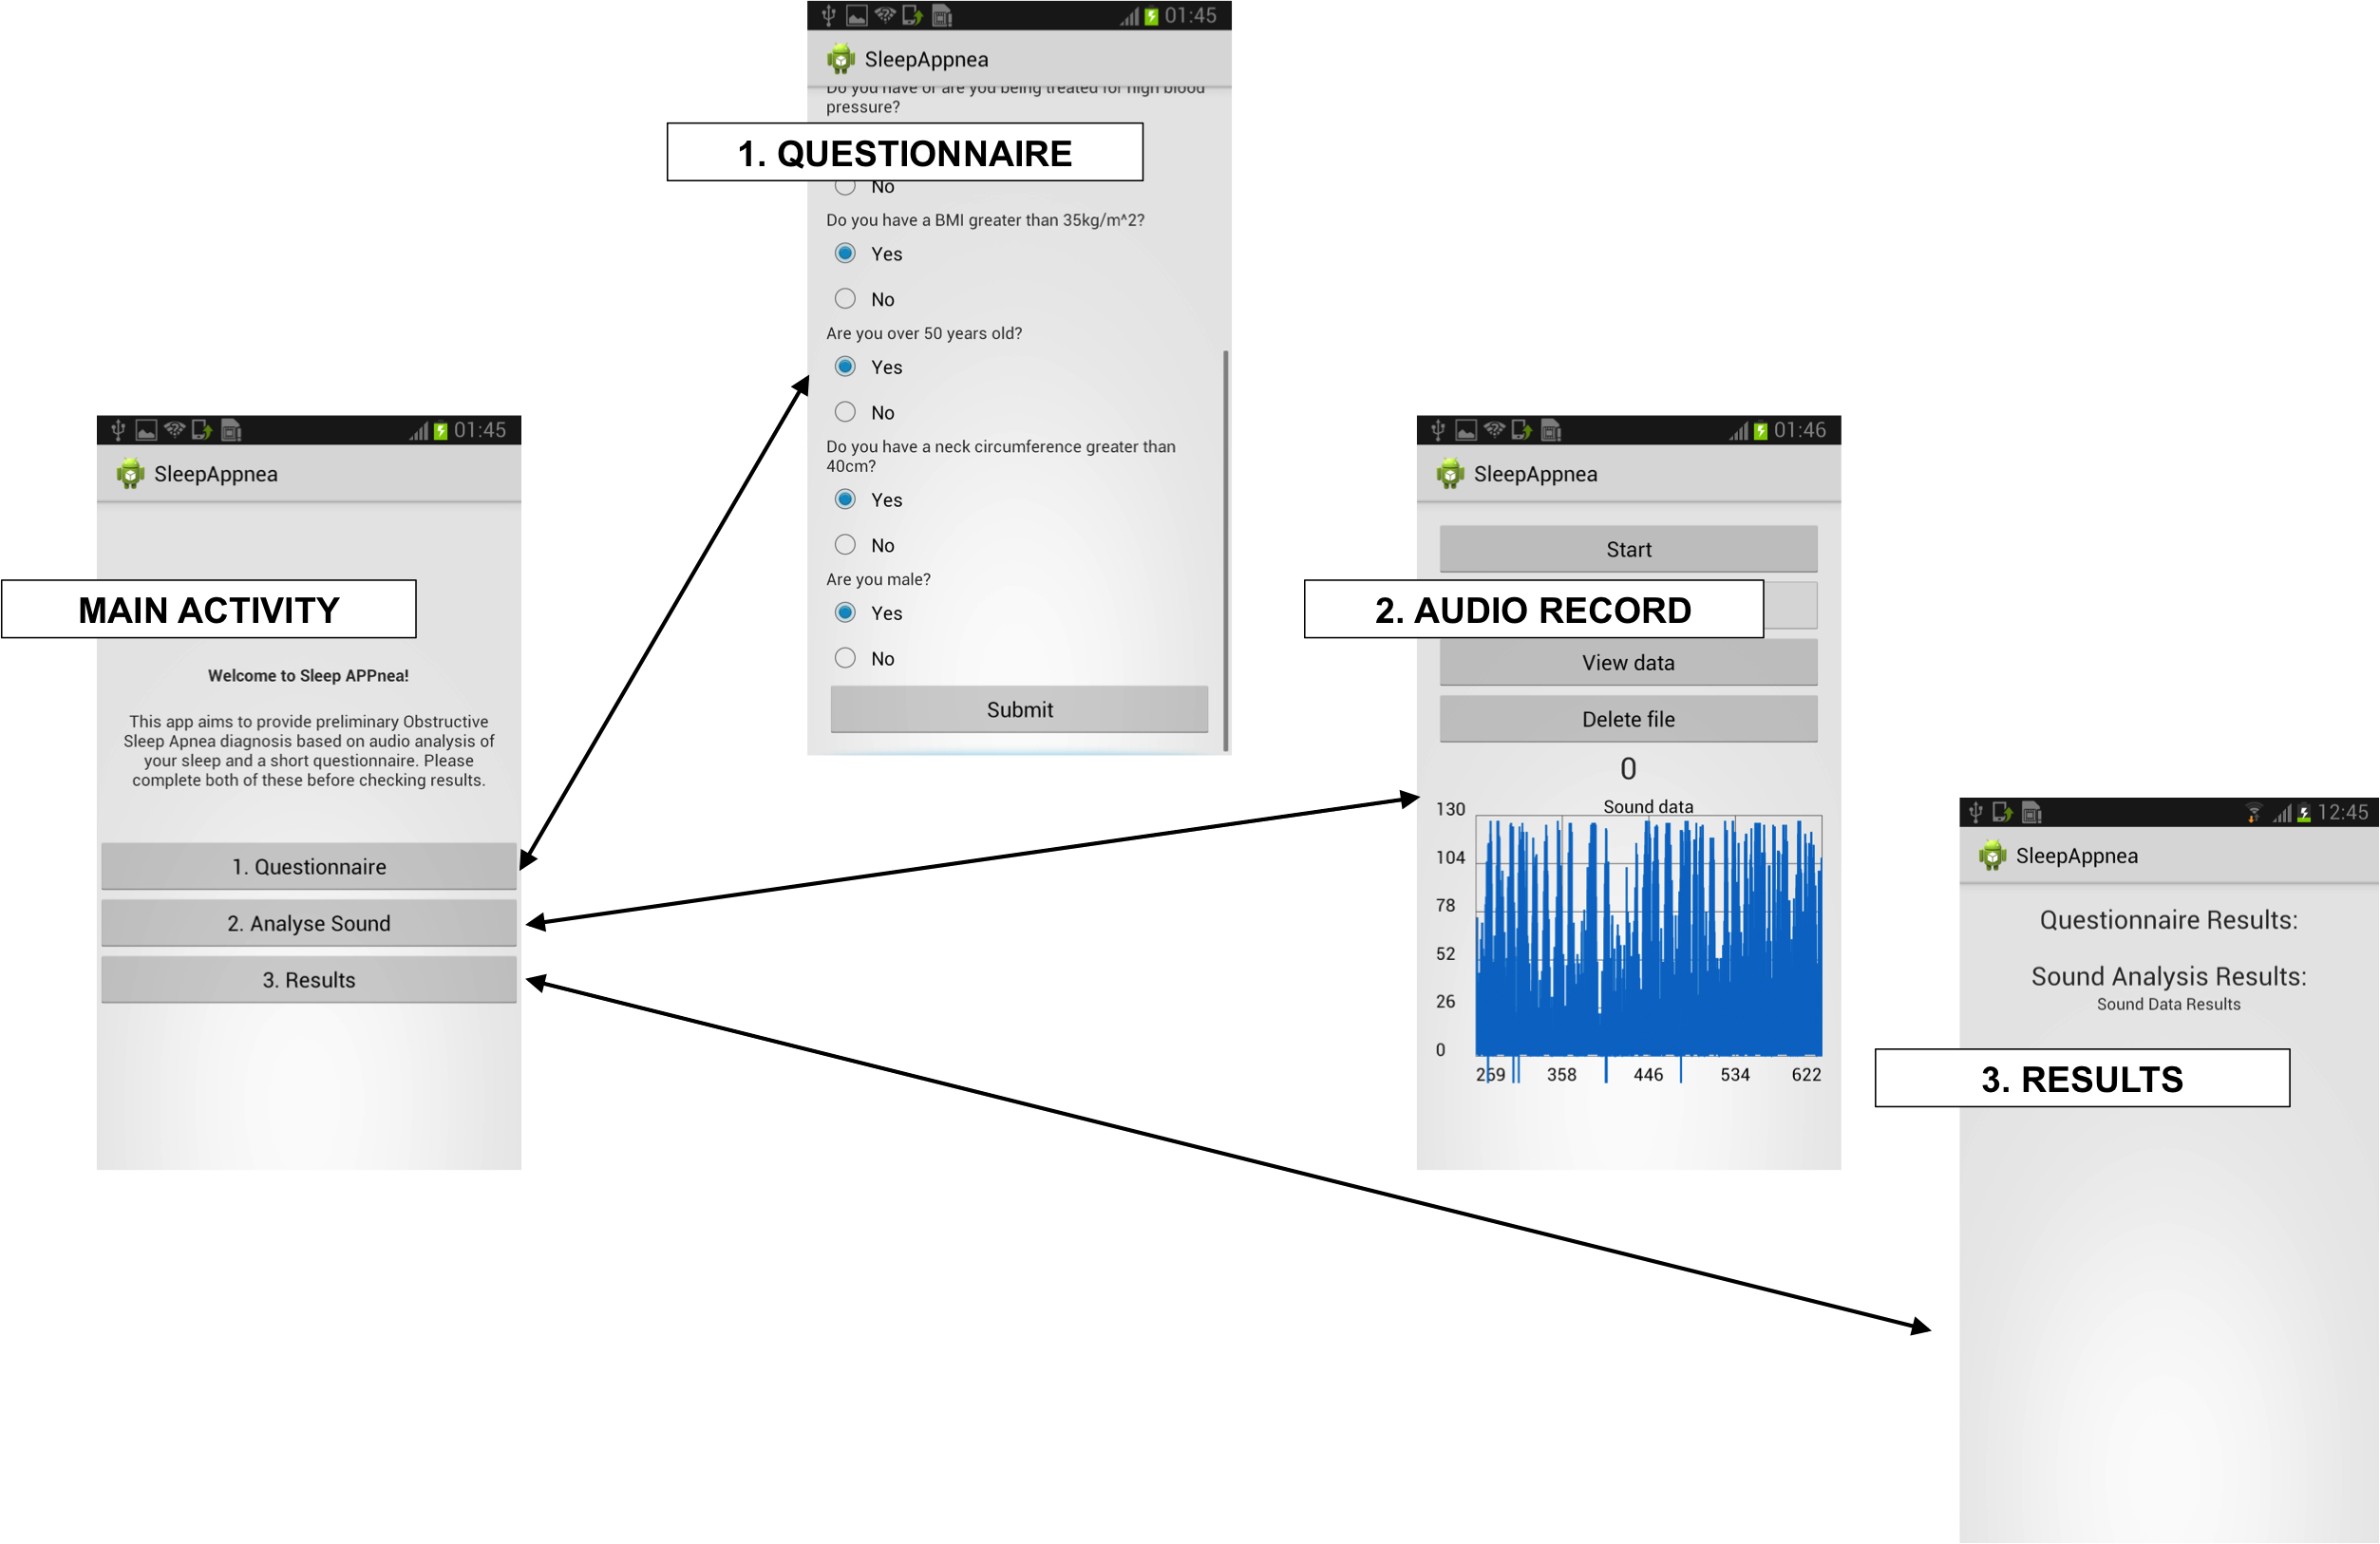
\includegraphics[width=.9\textwidth]{drawings/App_nav.png}
		\caption{Navigation between home activity and other pages}
		\label{fig:appStructure}
	\end{figure}
\subsection{Home Activity}
The app loads into the home activity when it is first turned on. The user is welcomed to the app and given a brief explanation of how to use the app. Below this the user is presented with three buttons to launch the three other activities. 
\subsection{Questionnaire Activity}
The first task for the user to complete is the questionnaire, based on the eight STOPBANG criteria questions as detailed later in the ‘Design Process’ section of this report. Pressing the submit button then takes you back to the start page and simply stores the number of ‘yes’ answers the questionnaire received. This number is called during the processing of the overall results, noting that three or more ‘yes’ answers indicates a high risk of Obstructive Sleep Apnea. The default for all of the answers is ‘yes’ which should encourage the user to actively read/change each question (given that statistically the average person would have more ‘no’ answers). It also means that should the user bypass the questionnaire section or ignore the questions before hitting ‘submit’, the app will use the higher risk criteria and results will be more likely to suggest too high a probability of apnea than miss a positive diagnosis altogether. 
\subsection{Sound Analysis Activity}
This activity is indicated as the second task to complete, though it doesn’t require completion of the questionnaire before being executable itself. The user is presented with four simple buttons as seen below. Note the following button restrictions (Figure \ref{fig:recordPages}):
\begin{itemize}
\item `Stop' cannot be pressed until the phone is recording audio.
\item `View Data' and ‘Delete File’ do nothing until there is data stored (‘Nothing yet’ is displayed as an indicator’).
\item When `Start' has been pressed, the ‘Stop’ button becomes the only usable button. This is done by checking whether the inbuilt Boolean variable ‘isRecording’ is true, and as such, the inverse becomes true again as soon as ‘Stop’ is pressed.
\end{itemize}
\begin{figure}[ht!]
		\centering
			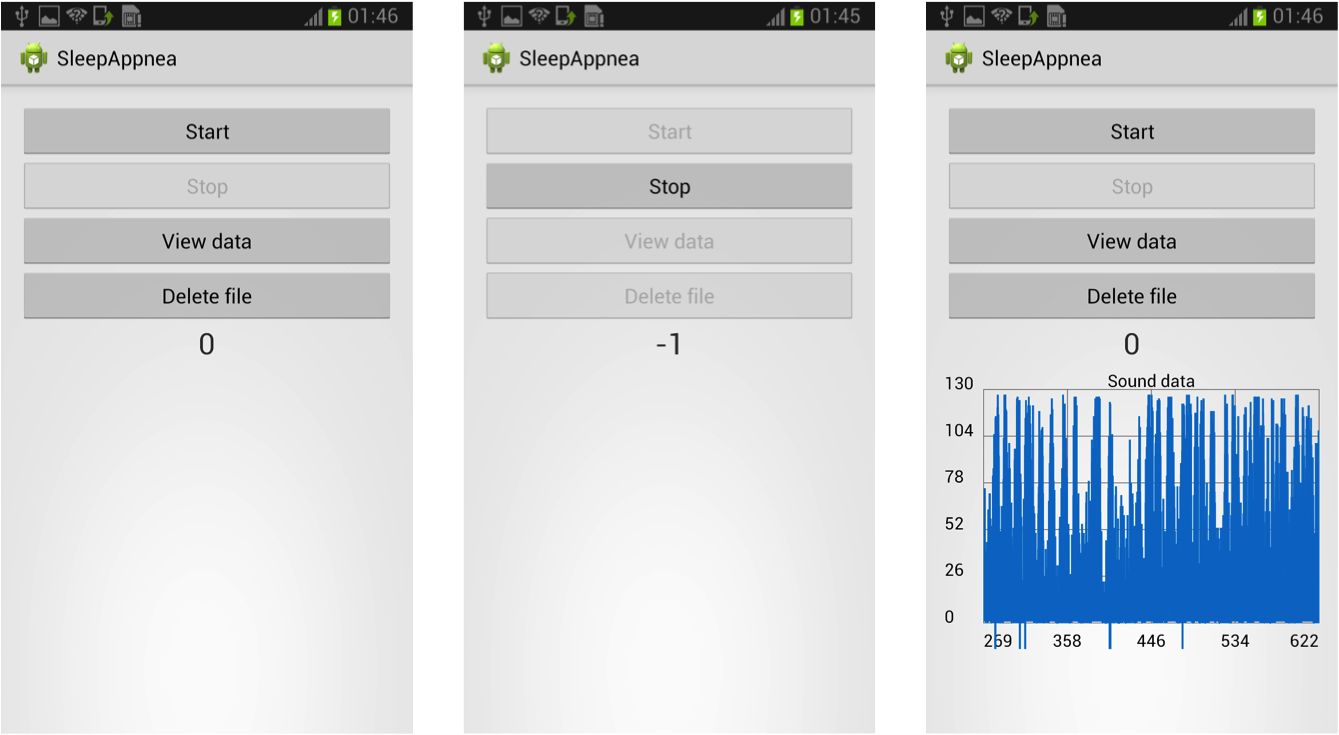
\includegraphics[width=.9\textwidth]{drawings/Audiorecord_struct.png}
		\caption{Buttons are disabled depending on whether recording is in process}
		\label{fig:recordPages}
	\end{figure}
(see Figure \ref{fig:recordPages})
For this simple prototype of the app, recording is restricted to one file in any instance of the app running.
\\ The sound data is automatically stored to a file accessible only by the app and is later analyzed by the machine-learning algorithm and overall results algorithm. Clearly the delete button is only included for cases where recordings were accidentally created and as such, it uses a comprehensive ``Are you sure?'' alert upon pressing to avoid deletion of wanted files.
\\Progress bars are used whilst the sound is being saved and loaded which will reassure the user that the app is still running properly during these otherwise unresponsive stages of high CPU usage. 
\subsection{Results Activity}
In this activity, a simple algorithm is used to determine an overall probability that the user has obstructive sleep apnea, and brief medical advice is given accordingly. It combines the results of the questionnaire and the audio recording analysis to do this, and therefore if one of these two parts is not present, it will ask for the user to go back and complete it before full results are displayed. Again, all analysis and loading tasks that takes more than half a second or so utilize a progress bar for improved user interface.
\subsection{Navigation Around The App}
The buttons are intended to be as intuitive as possible for navigation of the app. Loading each extra activity can only be done from the home activity, and the activity is exited by pressing the hardware ``back'' button whilst on the home activity (see Figure \ref{fig:nativeButtons}). Each extra activity exits back to the home activity upon pressing this ``back'' button too, though the Questionnaire has the same functionality added in to the ``Submit'' button which helps reassure the user that the button has indeed been pressed.
\begin{figure}[ht!]
		\centering
			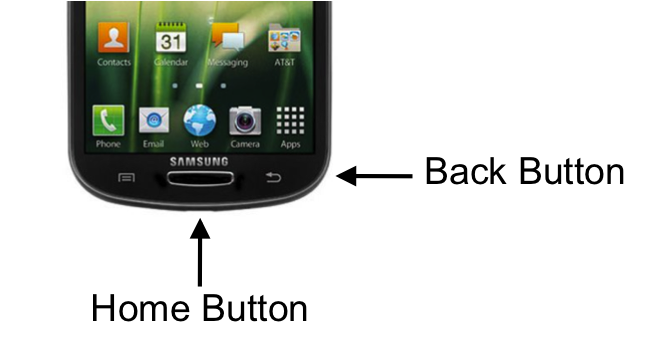
\includegraphics[width=.5\textwidth]{drawings/android_buttons.png}
		\caption{The hardware buttons are also coded for intuitive navigation}
		\label{fig:nativeButtons}
	\end{figure}